\chapter{Soft Argumentation Framework (Weighted AF)}
\section{Definizione di Soft Argumentation Framework}
Un Soft Argumentation Framework è una quadrupla:
\begin{center}
    $(A_{rgs} , R, W, S)$
\end{center}
dove:
\begin{itemize}
    \item $A_{rgs}$ è un insieme di Argomenti.
    \item R è una relazione di attacco sugli argomenti in $A_{rgs}$.
    \item W : $A_{rgs}$ x $A_{rgs}$ $\rightarrow$ S è una funzione binaria che
          rappresenta il peso associato ad ogni arco.
    \item S è un semiring $< A, +, x, bottom, top >$ Dati a, b $\in$ Args ,
          $\forall$(a, b) $\in$ R, W (a, b) = s significa che a attacca b con un peso
          di s $\in$ S.
\end{itemize}

\textbf{ Esempio:}
\begin{figure}[H]
    \centering
    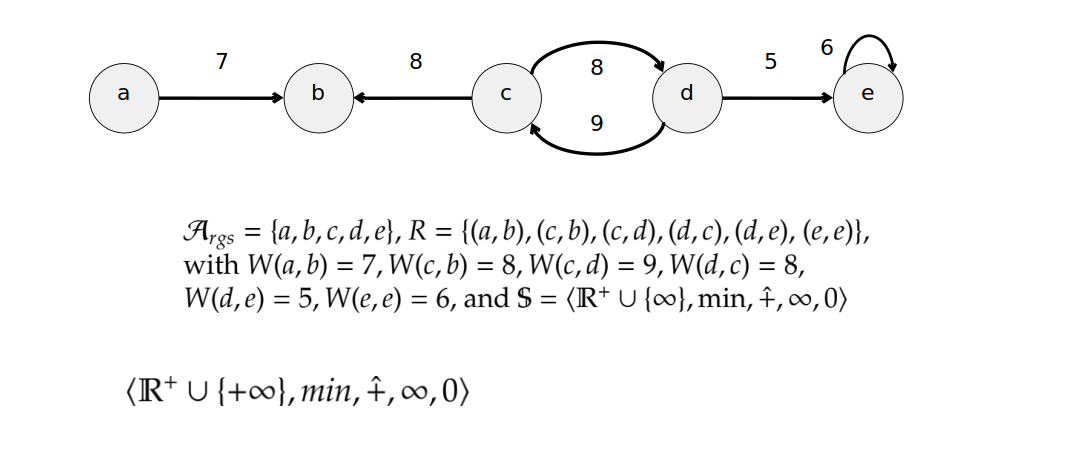
\includegraphics[width=14cm, keepaspectratio]{capitoli/img/Cap6/SoftA2.png}
\end{figure}

\textbf{Cambia la nozione di attacco:} Prima l'attacco era una funzione
booleana (a attacca b). Adesso invece quando a attacca b gli viene associato un
valore (comunque appartenente al semiring). \\\textbf{Cambia la nozione di
    difesa:} Nell'esempio sopra, nel caso in cui fossimo negli AF tradizionali C si
difenderebbe dall'attacco di D (perché ricordiamo era una funzione booleana). In
questo caso però, essendo che d attacca c con 9 e c risponde con 8, c non potrà
difendersi dall'attacco, poiché la difesa non è sufficiente a contrastare
quest'ultimo. Questa nozione dipende strettamente dal semiring utilizzato,
poiché per ogni semiring (i cui tipi sono gli stessi introdotti precedentemente)
si avranno relazioni diverse.
\section{w-difesa (Dw)}
Dato un Soft Argumentation Framework $(A_{rgs} , R, W, S)$, un sottoinsieme di
argomenti B $\subseteq$ Args w-difende un argomento b $\in$ Args se e soltanto
se, dato a $\in$ Args tale per cui R(a, b), allora:
\begin{center}
    $W (a, B \cup \{b\}) >=_s s W (B, a)$
\end{center}
L'insieme B w-difende l'elemento b se e soltanto se difende b da tutti gli
attacchi che arrivano a b cioè da tutti gli R(a, b). \\$>=_S$ è da intendere
    come elemento migliore o peggiore all'interno del semiring. \\In altre parole,
    devo verificare che il peso degli attacchi che ricevo sia inferiore al peso
    degli attacchi che invio.
    \begin{itemize}
        \item Con W (a, B $\cup$ \{b\}) si intende il costo degli attacchi che
              vanno da a all'insieme B $\cup$ \{b\} (cioè tutti gli attacchi che
              apporta quell'elemento a all'insieme B "dall'esterno verso l'interno")
              sommati con l'operatore di combinazione del semiring. Per sapere quindi
              quanto vale l'attacco di a verso l'insieme B $\cup$ \{b\} nel caso di
              Semiring Weighted ad esempio devo fare la somma di tutti gli attacchi
              (proprio perché l'operatore di combinazione è la somma).
        \item W (B, a) sarebbe "con quanto l'insieme B attacca a, cioè tutti gli
              attacchi dall'interno di B all'esterno". Anche questo dipende
              strettamente dal semiring, nel Weighted vanno tutti sommati.
    \end{itemize}
    \textbf{Esempio}
    \begin{figure}[htp]
        \centering
        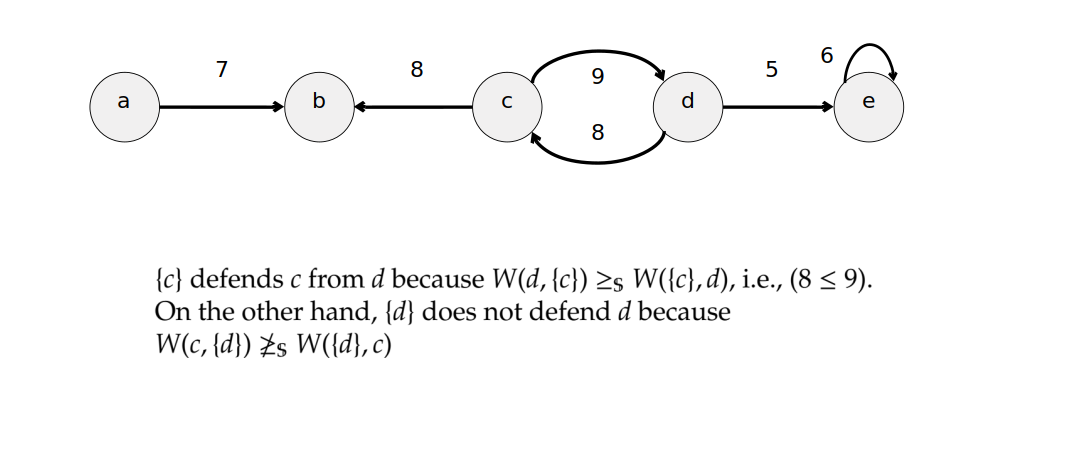
\includegraphics[width=14cm, keepaspectratio]{capitoli/img/Cap6/srs2.png}
    \end{figure}
    \\Per il calcolo degli insiemi ammissibili esistono vari metodi, che variano
    in base a regole imposte da autori di articoli scientifici.

    \section{Estensioni nei Weighted AF}
    \subsection{w-Conflict Free}
    Dato un W F = $(A_{rgs} , R, W, S)$, un sottoinsieme di argomenti B
$\subseteq$ Args è w-conflict free se e soltanto se W(B, B) = top (top del
    semiring). Questo significa che nessuno degli elementi dentro l'insieme
    attacca un altro elemento sempre dentro l'insieme. Dire che il peso è uguale
    al top del semiring (o al bottom) significa che quel peso non è presente, e
    quindi non è presente una relazione di attacco.
    \subsection{w-Admissible}
    Dato un W F = $(A_{rgs} , R, W, S)$, un insieme di argomenti B $\subseteq$
    Args w-conflict-free è w-admissible se e soltanto se tutti gli argomenti di
    B sono w-difesi da B.
    \section{Distinzione tra gli insiemi Admissible}
    \subsection{Martinez e Simari (D1)}
    L'obiettivo è capire se l'insieme B = \{b, c, d, e\} riesce a difendersi
    dall'attacco di a e poi dall'attacco di f , cioè se quell'insieme è
    ammissibile. Prendiamo in considerazione per tutti il semiring Weighted.
    Secondo Martinez e Simari non si aggregano ne le difese ne gli attacchi,
    quindi prendo il massimo degli attacchi ed il massimo delle difese.
    \begin{figure}[htp]
        \centering
        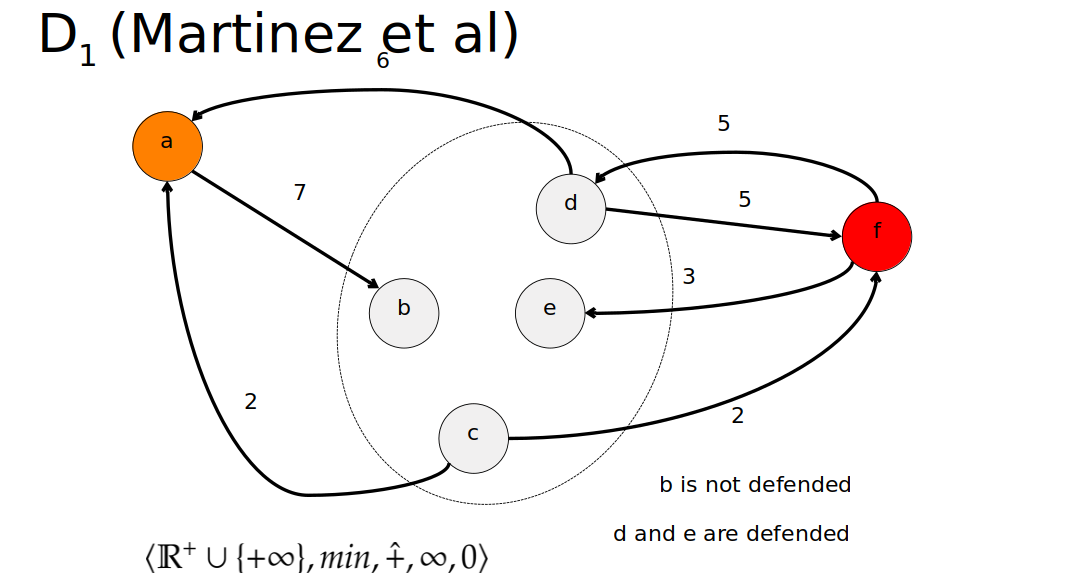
\includegraphics[width=13cm, keepaspectratio]{capitoli/img/Cap6/martinez2.png}

    \end{figure}
    \\\textbf{Esempio:} Devo verificare che il \textbf{massimo} valore degli
    \textbf{attacchi} sia maggiore del \textbf{massimo} valore delle
    \textbf{difese}. \\\textbf{Attacco} di a \textbf{verso} b:
    \begin{itemize}
        \item Attaccanti (a): Max(7) = 7
        \item Difensori (d,c): Max(6,2) = 6
        \item Conclusione: 6 $<$ 7, b non è difeso e quindi non ammissibile
    \end{itemize}
    \textbf{Attacco} di f \textbf{verso} d, e:
    \begin{itemize}
        \item  Attaccanti (f): Max(5,3) = 5
        \item Difensori (d,e): Max(5,2) = 5 (il 2 viene dall'attacco di c verso
              f)
        \item Conclusione: 5 = 5, (d), (e) sono difesi e quindi ammissibili.
    \end{itemize}
    La nozione formale di difesa in Simari-Martinez è: Dato W F = $(A_{rgs} , R,
W, S)$, a, b, c $\in$ $A_{rgs}$ , B $\subseteq$ $A_{rgs}$ , allora b è
    difeso da B se per ogni R(a, b), esiste almeno uno c $\in$ B tale per cui W
    (a, b) $>=_s$ W (c, a).


    \subsection{Coste-Marquis (D2)}
    Questo approccio aggrega solamente le \textbf{difese.}
    \begin{figure}[htp]
        \centering
        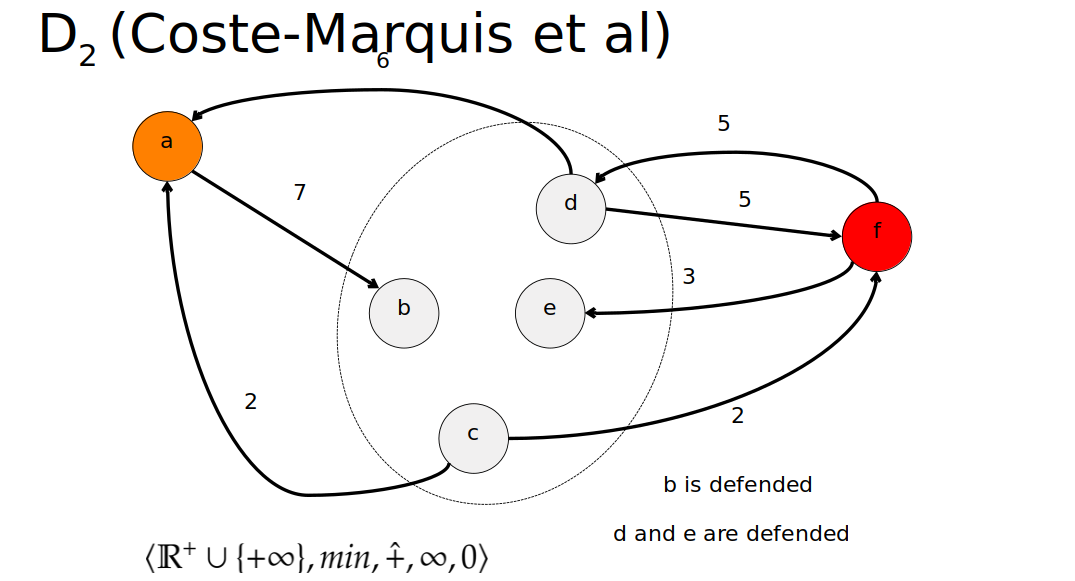
\includegraphics[width=13cm, keepaspectratio]{capitoli/img/Cap6/marquis2.png}
    \end{figure}
    \\\textbf{Attacco} di a \textbf{verso} b:
    \begin{itemize}
        \item Attaccanti (a): Max(7) = 7
        \item Difensori (d,c): Difesa(6)+Difesa(2) = 6+2 = 8
        \item Conclusione: 8 $>$ 7, b è difeso e quindi ammissibile
    \end{itemize}

    \subsection{Santini e Bistarelli (Dw)}
    Questo approccio aggrega \textbf{sia gli attacchi che le difese, ciò vuol
        dire che b è difeso ma d ed e no.}

    \begin{figure}[htp]
        \centering
        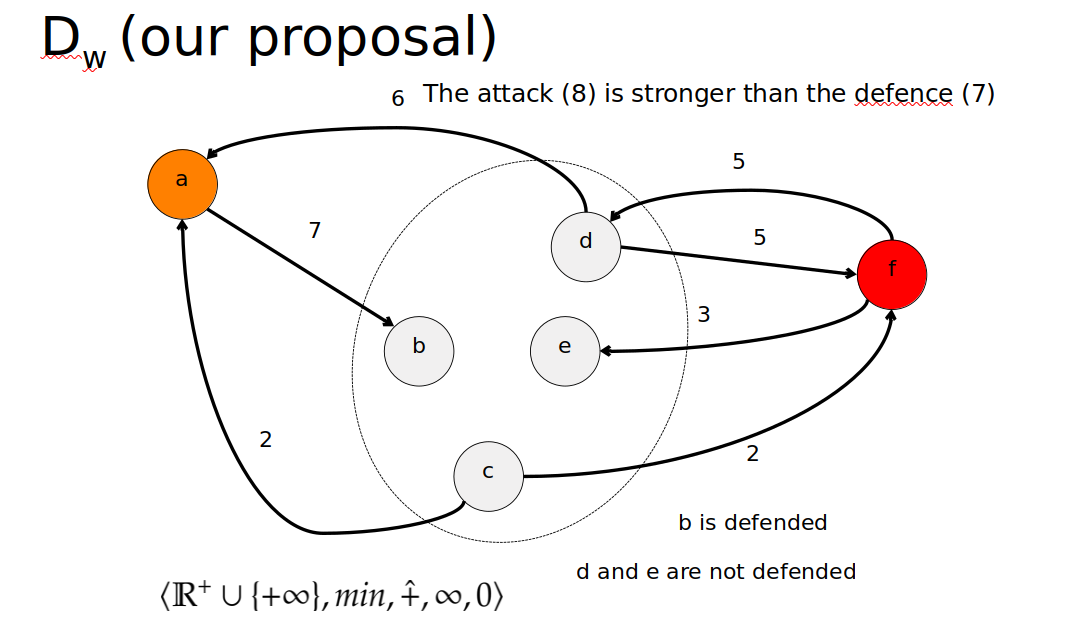
\includegraphics[width=13cm, keepaspectratio]{capitoli/img/Cap6/bistarelli2.png}
    \end{figure}

    \textbf{Attacco} di a \textbf{verso b:}

    \begin{itemize}
        \item Attaccanti (a): Attacco(7) = 7
        \item Difensori (d,c): Difesa(6)+Difesa(2) = 6+2 = 8
        \item Conclusione: 8 $>$ 7, b è difeso e quindi ammissibile
    \end{itemize}
    \textbf{Attacco} di f \textbf{verso d, e:}
    \begin{itemize}
        \item Attaccanti (f): Attacco(5)+Attacco(3) = 5+3 = 8
        \item Difensori (d,e): Difesa(5) + Difesa(2) = 7
        \item Conclusione: 8 $>$ 7, d, e \textbf{non} sono difesi e quindi non
              ammissibili.
    \end{itemize}

    \subsection{Teoremi di implicazione tra le nozioni}
    \textbf{N.B1 (da sapere):} La relazione di w-difesa implica la relazione di
    difesa:
    \begin{center}
        B w-difende b $\rightarrow$ B difende b
    \end{center}
    \textbf{N.B2:} Nel semiring Classic (booleano) si ha che:
    \begin{center}
        B w-difende a $\Leftarrow \Rightarrow$ B difende a
    \end{center}
    \begin{itemize}
        \item $D_W$ $\Rightarrow$ $D_2$ , Bista implica Costa-Marquis
        \item $D_1$ $\Rightarrow$ $D_2$ , Martinez implica Costa-Marquis
        \item Quindi se è ammissibile per Martinez e Bista allora è ammissibile
              anche per Costa-Marquiz
        \item Se S $=< [0, 1], max, min, 0, 1 > $ cioè semiring Fuzzy, allora D1
              $\Leftarrow \Rightarrow$ D2
        \item Se $S =< [0, 1], max, min, 0, 1 >$ cioè semiring Fuzzy, allora Dw
              $\Leftarrow \Rightarrow$ D1
        \item Se $S =< [true, false], or, and, false, true >$ cioè semiring
              Classic, \\allora $D_w \Leftarrow \Rightarrow D_0 \Leftarrow
                  \Rightarrow D1 \Leftarrow \Rightarrow D_2$ (ma cosa è $D_0$ )??
    \end{itemize}
    \begin{figure}[H]
        \centering
        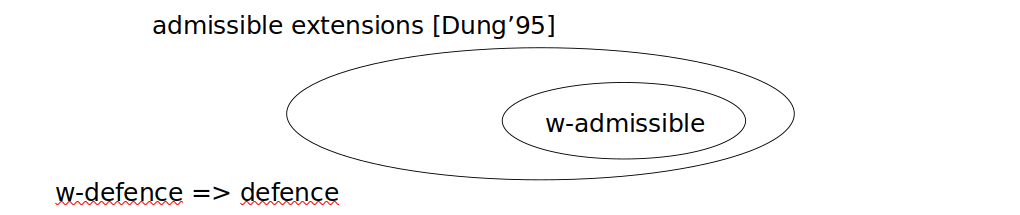
\includegraphics[width=14cm, keepaspectratio]{capitoli/img/Cap6/teor1.png}
        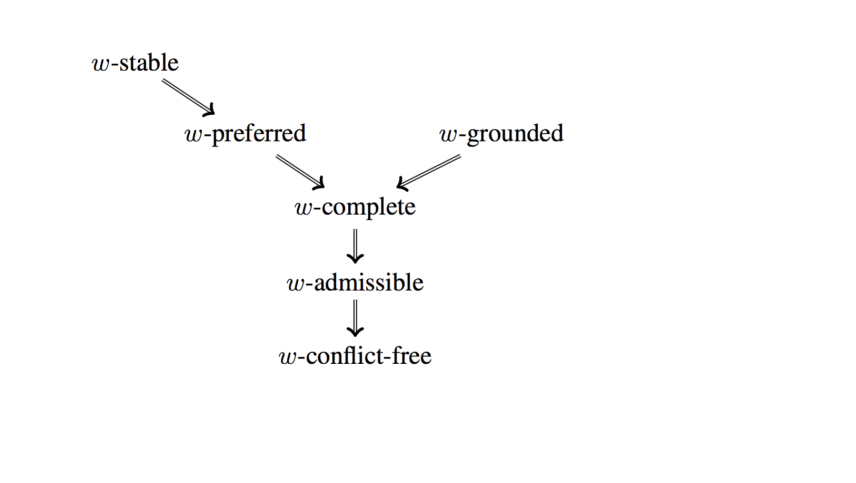
\includegraphics[width=14cm, keepaspectratio]{capitoli/img/Cap6/teor2.png}
    \end{figure}
    L'implicazione delle semantiche è la stessa sia nel caso classico che in
    quello pesato.

    \section{Orthogonal Relaxations}
    \begin{figure}[H]
        \centering
        
\includegraphics[width=14cm, keepaspectratio]{capitoli/img/Cap6/ortogonal.png}
    \end{figure}
    \noindent In questo esempio notiamo che (d, c) non stanno bene insieme,
    perché si attaccato 100. (b, c) sono abbastanza compatibili, perché la
    relazione di attacco è presente ma con peso molto basso. Abbiamo poi che b
    non è ammissibile (non riesce a difendersi da c), c è ammissibile, d è
    ammissibile e nessuna coppia di argomenti è ammissibile. Questo però non è
    una cosa positiva, perché si vorrebbero cercare delle coalizioni superiori
    al singleton. Se però riuscissi ad accettare un po' di conflitti interni
    potrei comunque creare una coalizione. Infatti notiamo che potremmo mettere
    insieme (b, c) dato che la relazione di attacco è si presente ma con peso
    molto basso. Introduciamo quindi l'Alpha-gamma consistenza.\\
    Questi rilassamenti sono strettamente correlati e influenzano l'un l'altro:
    permettere un piccolo conflitto può portare ad avere più argomentazioni in
    un'estensione, e di conseguenza si ha una difesa più forte o più debole. Un
    esempio reale potrebbe essere in campo politico, partiti con piccole
    divergenze interne si uniscono in modo da raggiungere una percentuale
    sufficiente di voti per governare.

    \section{Alpha-Gamma consistenza}
    Che cosa è l'\textbf{alpha-gamma consistenza?} \\ Questa consistenza
    definisce il quantitativo di attacchi "interni" cioè alpha ed ”esterni” cioè
    gamma che si ammettono.
    \begin{figure}[htp]
        \centering
        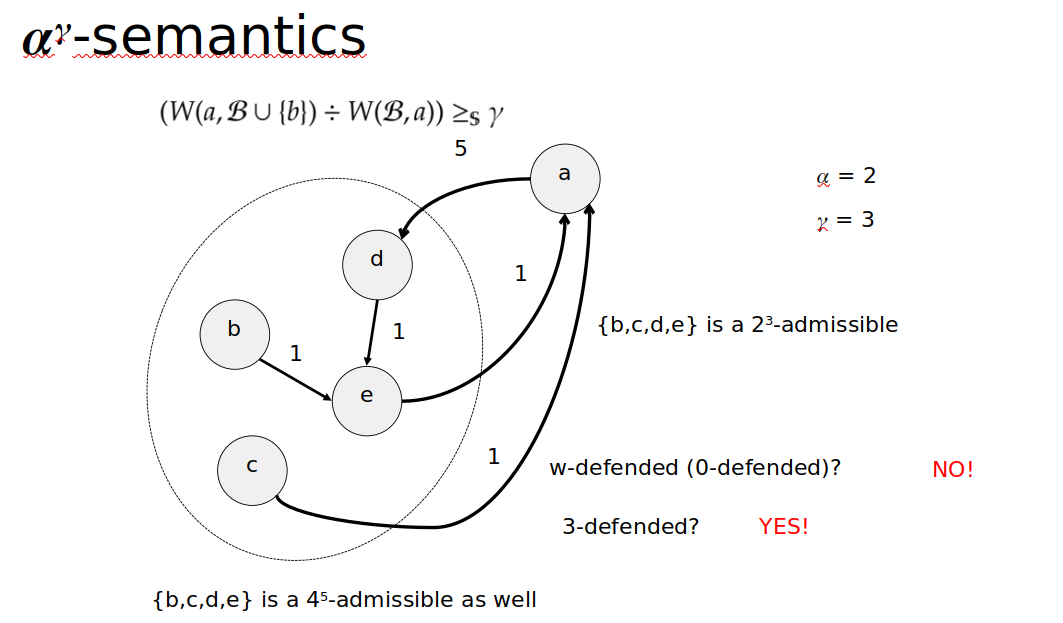
\includegraphics[width=12cm, keepaspectratio]{capitoli/img/Cap6/cons2.png}
    \end{figure}
    \\In questo esempio, l'insieme $B = \{b, c, d, e\}$ non è conflict-free (b e
    d attaccano e), però se volessimo misurare il valore di questo conflitto
    considerando il semiring Weighted (operazione somma), l'insieme è
    2-conflict-free (infatti 2 elementi in questo insieme attaccano un altro
    elemento sempre appartenente all'insieme). Se quindi la soglia $\alpha$
    fosse 2 riuscirei a sopportare l'attacco tramite il rilassamento dei
    conflitti interni. Guardiamo l'ammissibilità dell'insieme: a attacca
    l'insieme B con 5 e B è difeso da 1 ed 1. In realtà l'argomento d andrebbe
    escluso dall'insieme perché porta un attacco con peso molto alto all'insieme
    stesso. Se però devo per forza costruire un organo di 4 elementi devo
    accettare sia i conflitti interni sia l'attacco verso d (potrei anche
    portare dentro a).

    \subsection{Unità di sopportazione \texorpdfstring{$\gamma$}{gamma}}
    \textbf{N.B} secondo Bistarelli l'insieme B non è ammissibile, perché
    l'attacco di 5 non è difeso dalla somma delle difese 1+1=2. Facendo il
    calcolo: (attacco-difesa) 5-2=3 si calcola l'unità di \textbf{sopportazione}
$\gamma$ che in questo caso è 3. \\Quindi:
    \begin{itemize}
        \item $\alpha$ Peso del \textbf{conflitto interno} (in questo caso 2,
              dall'attacco di b pari ad 1 e d sempre 1 verso e)
        \item $\gamma$ Peso del \textbf{conflitto esterno} (in questo caso 3 (5
              - 2))
    \end{itemize}
    L'insieme dell'esempio sopra è $2^3$ \textbf{admissible} perché $\alpha$ = 2
    e $\gamma$ = 3. Inoltre B è anche stabile, perché tutti gli elementi esterni
    (in questo caso solo a) sono attaccati. Nel caso in cui portassimo d fuori
    si avrebbe un valore più basso di $\gamma$ ma B non sarebbe stato stabile,
    perché nessuno attaccava d (a rimaneva comunque fuori). \\
    La semantica Alpha Gamma può essere descritta come:
    \begin{center}
        $W (a, B \cup \{b\}) \div W (B, a)) >=_s \gamma$
    \end{center}
    dove:
    \begin{itemize}
        \item $W (a, B \cup \{b\})$ : Il peso dell'attacco dall'esterno a verso
              l'interno B
        \item $\div$ : opposto della combinazione (x), abbiamo fatto esempi
              sempre con il Weighted, cioè la somma, quindi assumiamo sia la
              \textbf{sottrazione}
        \item W (B, a) Il peso dell'attacco dall'interno B verso l'esterno a
        \item Il risultato deve essere $>=_s$ $\gamma$ (migliore all'interno del
              semiring s).
    \end{itemize}
    L'insieme $B = \{b, c, d, e\}$ è anche $4^5$ \textbf{admissible}, e per
    dimostrare questo facciamo riferimento alle inclusioni.

    \subsection{Inclusioni in Alpha-Gamma consistenza}
    \textbf{Teorema}: Dato un W F=$(A_{rgs }, R, W, S)$ con S=$(A, (+), (x),
bottom, top)$ e $\alpha, \gamma \in$ A:
    \begin{center}
        $\alpha^\gamma-stable \rightarrow \alpha^\gamma-prefered \rightarrow
            \alpha^\gamma-complete \rightarrow \alpha^\gamma-admissible \rightarrow
            \alpha-conflict-free$
    \end{center}
    \begin{figure}[htp]
        \centering
        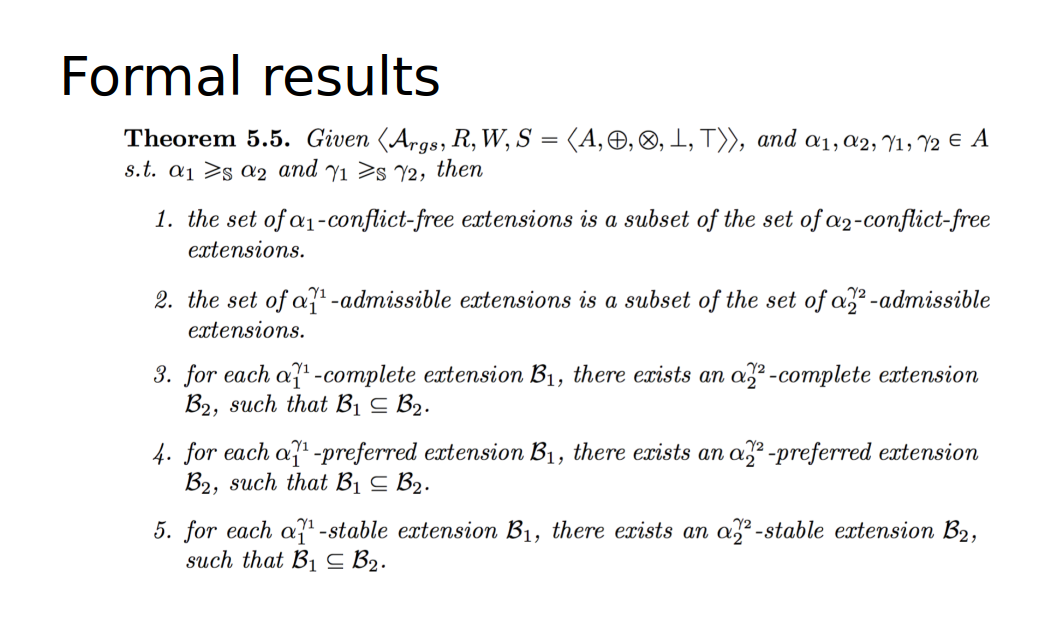
\includegraphics[width=15cm, keepaspectratio]{capitoli/img/Cap6/alpha-gamma2.png}
    \end{figure}
    \textbf{Le uniche cose spiegate dal prof nella figura sopra sono:}
    \\Se un estensione è $ \alpha_1$ ammissibile e $\alpha_1 >=_s \alpha_2$
    allora quell'estensione è anche $\alpha_2$ ammissibile. Stessa cosa per
$\gamma$. \\Questo significa che nell'esempio sopra che era $2^3$ admissible
    sarà anche $4^5$ ammissibile (ecco spiegata la domanda della sezione sopra).

\section{w-Grounded}
Gli insiemi grounded sono gli insiemi complete più piccoli. \\\textbf{Def di
    Grounded (Minimale) nel caso normale (Crisp AF):}
\begin{center}
    E $\in$ gr(F) if f E $\in$ co(F) e \textbf{non esiste} E' $\in$ co(f)
    tale per cui E' \textbf{non è contenuto} in E.
\end{center}
Un estensione E è grounded se e solo se è una complete e nessun altra
estensione dentro le complete è più piccola di lei (quindi è la più piccola
delle complete).
\begin{figure}[H]
    \centering
    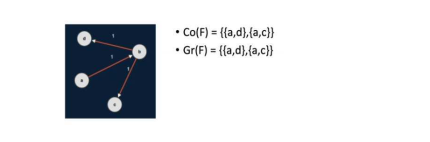
\includegraphics[width=14cm, keepaspectratio]{capitoli/img/Cap6/w-grounded.png}
\end{figure}

\textbf{Calcolo delle complete se non ci fossero i pesi:} L'insieme
complete era (a, d, c) perché a difendeva sia d che c insieme.
\\\textbf{Calcolo delle complete con pesi (usiamo Bistarelli):} Le complete
in questo caso sono a perché non viene attaccata da nessuno e più tutte
quelle difese da a cioè d e c. \textbf{Non le difende tutte e due insieme}
perché il costo 1 non è sufficiente e difenderle tutte e due, deve per forza
farlo uno alla volta (cosi ha detto il bista). Quindi le complete sono (a,
d) e (a, c). Applicando la definizione di Grounded all'esempio otteniamo che
l'insieme è sempre lo stesso delle complete, ma questo è un problema, perché
le grounded hanno la proprietà di essere \textbf{uniche}. \\\textbf{Tutto
    quello sopra è per dimostrare che la definizione di Grounded con pesi negli
    AF va cambiata a}:\\
Un elemento E è Grounded se e soltanto se:
\begin{enumerate}
    \item \textbf{ É ammissibile} (prima si richiedeva che era complete);
    \item  É incluso nell'intersezione delle \textbf{complete};
    \item  Non esiste nessun elemento \textbf{ammissibile} più grande di E.
\end{enumerate}
\begin{figure}[htp]
    \centering
    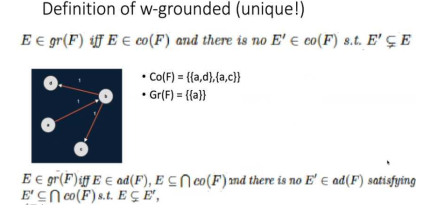
\includegraphics[width=12cm, keepaspectratio]{capitoli/img/Cap6/w-gounded2.png}
\end{figure}
L'insieme degli ammissibili in questo caso era: (a), (a, c), (a, d) quindi
l'intersezione viene a che è appunto l'unica grounded (e non è attaccata da
nessuno). \\Negli Weighted AF la definizione di Grounded va cambiata perché
altrimenti si perderebbe la proprietà di essere \textbf{uniche}.
\section{Argomento Scetticamente/Credulosamente accettato}
Trattiamo adesso un problema decisionale (quindi chiedere se un argomento è
SI/NO), introducendo il significato di un argomento Credulosamente o
\textbf{Skep/(Scet)ticamente }accettato su questo esempio.
\begin{figure}[htp]
    \centering
    
\includegraphics[width=14cm, keepaspectratio]{capitoli/img/Cap6/scet.png}
\end{figure}
\begin{itemize}
    \item \textbf{Cred} (Almeno in un insieme): Ci domandiamo: esiste
          \textbf{almeno} una volta che l'argomento 2 compare in output? La
          domanda va posta in base a quello che calcoliamo, ad esempio, nel caso
          in cui calcolassimo le conflict-free e il 2 non compare tra le coppie
          che lo sono, la risposta sarà NO, mentre nel caso in cui comparisse in
          almeno una coppia (o anche da solo) la risposta sarebbe SI.
    \item \textbf{Skept} (In tutti gli insiemi): Se un elemento è
          \textbf{sempre} dentro un estensione. In questo caso l'output sarà NO
          perché non c'è un elemento che è comune a tutti gli insiemi. É possibile
          selezionare l'elemento, quindi magari per il valore 4 da NO, ma per il
          valore 3 da SI.
\end{itemize}
